
%(BEGIN_QUESTION)
% Copyright 2013, Tony R. Kuphaldt, released under the Creative Commons Attribution License (v 1.0)
% This means you may do almost anything with this work of mine, so long as you give me proper credit

Calculate all resistor voltages and currents in these two circuits, also labeling all voltage polarities (+ and $-$ symbols) next to each component in both circuits:

$$\includegraphics[width=15.5cm]{i02769x01.eps}$$

% No blank lines allowed between lines of an \halign structure!
% I use comments (%) instead, so that TeX doesn't choke.

$$\vbox{\offinterlineskip
\halign{\strut
\vrule \quad\hfil # \ \hfil & 
\vrule \quad\hfil # \ \hfil & 
\vrule \quad\hfil # \ \hfil \vrule \cr
\noalign{\hrule}
%
% First row
Quantity & Series circuit & Parallel circuit \cr
%
\noalign{\hrule}
%
% Another row
$V_{R1}$ &  &  \cr
%
\noalign{\hrule}
%
% Another row
$V_{R2}$ &  &  \cr
%
\noalign{\hrule}
%
% Another row
$V_{R3}$ &  &  \cr
%
\noalign{\hrule}
%
% Another row
$I_{R1}$ &  &  \cr
%
\noalign{\hrule}
%
% Another row
$I_{R2}$ &  &  \cr
%
\noalign{\hrule}
%
% Another row
$I_{R3}$ &  &  \cr
%
\noalign{\hrule}
} % End of \halign 
}$$ % End of \vbox

\vskip 20pt \vbox{\hrule \hbox{\strut \vrule{} {\bf Suggestions for Socratic discussion} \vrule} \hrule}

\begin{itemize}
\item{} Predict the effects resulting from various wiring and component faults in this system (e.g. {\it opens} or {\it shorts}).
\item{} A useful analytical technique for any DC electric circuit is to identify all electrical sources and loads in the circuit, annotate the diagram with arrowheads showing the directions of all currents, and also with ``+'' and ``$-$'' symbols (and/or curved arrows) showing the polarities of all component voltages.  Show how this helps you analyze the circuit shown in this question.
\end{itemize}

\underbar{file i02769}
%(END_QUESTION)





%(BEGIN_ANSWER)

$$\includegraphics[width=15.5cm]{i02769x02.eps}$$

% No blank lines allowed between lines of an \halign structure!
% I use comments (%) instead, so that TeX doesn't choke.

$$\vbox{\offinterlineskip
\halign{\strut
\vrule \quad\hfil # \ \hfil & 
\vrule \quad\hfil # \ \hfil & 
\vrule \quad\hfil # \ \hfil \vrule \cr
\noalign{\hrule}
%
% First row
Quantity & Series circuit & Parallel circuit \cr
%
\noalign{\hrule}
%
% Another row
$V_{R1}$ & 2.722 V & 12 V \cr
%
\noalign{\hrule}
%
% Another row
$V_{R2}$ & 7.486 V & 12 V \cr
%
\noalign{\hrule}
%
% Another row
$V_{R3}$ & 1.792 V & 12 V \cr
%
\noalign{\hrule}
%
% Another row
$I_{R1}$ & 2.268 mA & 10 mA \cr
%
\noalign{\hrule}
%
% Another row
$I_{R2}$ & 2.268 mA & 3.636 mA \cr
%
\noalign{\hrule}
%
% Another row
$I_{R3}$ & 2.268 mA & 15.190 mA \cr
%
\noalign{\hrule}
} % End of \halign 
}$$ % End of \vbox


%(END_ANSWER)





%(BEGIN_NOTES)


%INDEX% Electronics review: series and parallel circuits

%(END_NOTES)


